\documentclass[UTF8,zihao=-4]{ctexart}
\usepackage[a4paper,top=2.0cm,bottom=2.0cm,left=2.2cm,right=2.2cm]{geometry}
\usepackage{amsmath,amssymb,booktabs,tabularx,array}
\usepackage{graphicx,float,caption}
\usepackage{xcolor,listings,tcolorbox}
\usepackage{fancyhdr,lastpage}
\usepackage[hidelinks]{hyperref}

\definecolor{navy}{HTML}{183B63}
\definecolor{blue}{HTML}{2B6EAE}
\definecolor{green}{HTML}{2F8F49}
\definecolor{orange}{HTML}{DF7615}
\definecolor{purple}{HTML}{7651B5}
\definecolor{soft}{HTML}{F3F7FB}
\definecolor{line}{HTML}{C9D4DF}
\definecolor{codebg}{HTML}{F6F8FA}
\definecolor{headergray}{HTML}{777777}

\hypersetup{
  pdftitle={系统开发工具基础 - 第2周实验报告},
  pdfauthor={朱元清},
  colorlinks=true,
  linkcolor=blue,
  urlcolor=blue
}

\pagestyle{fancy}
\fancyhf{}
\fancyhead[L]{\small\color{headergray}系统开发工具基础}
\fancyhead[R]{\small\color{headergray}第 2 周实验报告}
\fancyfoot[C]{\small\color{headergray}第 \thepage\ 页 / 共 \pageref{LastPage} 页}
\setlength{\headheight}{24pt}
\renewcommand{\headrulewidth}{0.5pt}
\renewcommand{\headrule}{\hbox to\headwidth{\color{line}\leaders\hrule height \headrulewidth\hfill}}

\lstdefinestyle{basecode}{
  basicstyle=\ttfamily\footnotesize,
  backgroundcolor=\color{codebg},
  frame=single,
  rulecolor=\color{line},
  breaklines=true,
  columns=fullflexible,
  keepspaces=true,
  showstringspaces=false,
  xleftmargin=0.3em,
  xrightmargin=0.3em,
  aboveskip=0.6em,
  belowskip=0.7em
}

\lstdefinestyle{shell}{style=basecode,language=bash}
\lstdefinestyle{python}{style=basecode,language=Python}
\lstdefinestyle{c}{style=basecode,language=C}
\lstdefinestyle{output}{style=basecode,language={}}

\newtcolorbox{summarybox}[1]{
  colback=soft,
  colframe=blue,
  boxrule=0.7pt,
  arc=2mm,
  title={#1},
  fonttitle=\bfseries,
  coltitle=navy
}

\newcommand{\experimentbanner}[3]{
  \begin{tcolorbox}[
    colback=soft,
    colframe=navy,
    boxrule=1pt,
    arc=2mm,
    left=4mm,right=4mm,top=2.5mm,bottom=2.5mm]
    \begin{tabularx}{\textwidth}{>{\Large\bfseries\color{navy}}p{2.7cm}X}
      实验#1 & {\large\bfseries\color{navy}#2}\quad{\normalsize（#3）}
    \end{tabularx}
  \end{tcolorbox}
}

\newcommand{\practicebanner}[2]{
  \begin{tcolorbox}[
    colback=soft,
    colframe=navy,
    boxrule=1pt,
    arc=2mm,
    left=4mm,right=4mm,top=2.5mm,bottom=2.5mm]
    \begin{tabularx}{\textwidth}{>{\Large\bfseries\color{navy}}p{2.7cm}X}
      实例 #1 & {\large\bfseries\color{navy}#2}
    \end{tabularx}
  \end{tcolorbox}
}

\captionsetup{font=small,labelfont=bf,labelsep=quad}
\setlength{\parindent}{2em}
\setlength{\parskip}{0.25em}

\begin{document}

\thispagestyle{fancy}
\vspace*{0.7cm}
\begin{center}
  {\fontsize{28}{34}\selectfont\bfseries 系统开发工具基础}\\[0.35cm]
  {\fontsize{22}{28}\selectfont 第 2 周实验报告}\\[1.0cm]
  {\Large 姓名：朱元清\qquad 学号：25020007193}\\[0.6cm]
  {\Large 2026 年 8 月 31 日}
\end{center}

\vspace{0.7cm}
\begin{tcolorbox}[
  colback=soft,
  colframe=navy,
  boxrule=0.8pt,
  arc=2mm,
  left=5mm,right=5mm,top=4mm,bottom=4mm]
  \centering
  \normalsize
  本报告记录第 2 周第 5--8 题的操作过程与验证结果，并补充 11 个课后练习实例。
  内容覆盖 Shell 进程与任务控制、开发环境与语言服务器、Python 调试与内存检测，
  以及基于性能分析的程序优化。
\end{tcolorbox}

\vspace{0.65cm}
\begin{table}[H]
  \centering
  \caption{第 2 周实验完成情况}
  \renewcommand{\arraystretch}{1.35}
  \begin{tabularx}{0.92\textwidth}{cX>{\raggedright\arraybackslash}p{4.6cm}c}
    \toprule
    题号 & 主题 & 关键工具 & 状态 \\
    \midrule
    5 & 控制一个可清理的后台任务 & Bash、jobs、信号与 trap & \textcolor{blue}{\checkmark\ 完成} \\
    6 & 语义重构与本地开发反馈 & Python 语言服务器、Ruff、pytest & \textcolor{green}{\checkmark\ 完成} \\
    7 & 用调试器定位归并排序缺陷 & pdb、pytest & \textcolor{orange}{\checkmark\ 完成} \\
    8 & 先测量，再优化慢速词频程序 & time、cProfile、set & \textcolor{purple}{\checkmark\ 完成} \\
    \bottomrule
  \end{tabularx}
\end{table}

\vfill
\experimentbanner{五}{控制一个可清理的后台任务}{进程、信号与任务控制}
\newpage

\subsection*{实验目标}
在前台启动脚本后，使用 \texttt{Ctrl-Z} 挂起任务，再通过 \texttt{bg}、\texttt{jobs}
和作业信息取得 PID；最后发送 \texttt{SIGTERM}，验证 trap 完成清理并正常退出。

\subsection*{脚本内容}
\lstinputlisting[style=shell]{../q05/worker.sh}

\subsection*{执行命令}
\begin{lstlisting}[style=shell]
cd q05
chmod +x worker.sh
rm -f stdout.log stderr.log cleanup.log
./worker.sh > stdout.log 2> stderr.log
# Press Ctrl-Z
bg
jobs
pid=$(jobs -l %1 | awk '{print $3}')
echo "$pid"
kill -TERM "$pid"
wait "$pid"
jobs
cat cleanup.log
cat stdout.log
cat stderr.log
\end{lstlisting}

\clearpage
\begin{figure}[H]
  \centering
  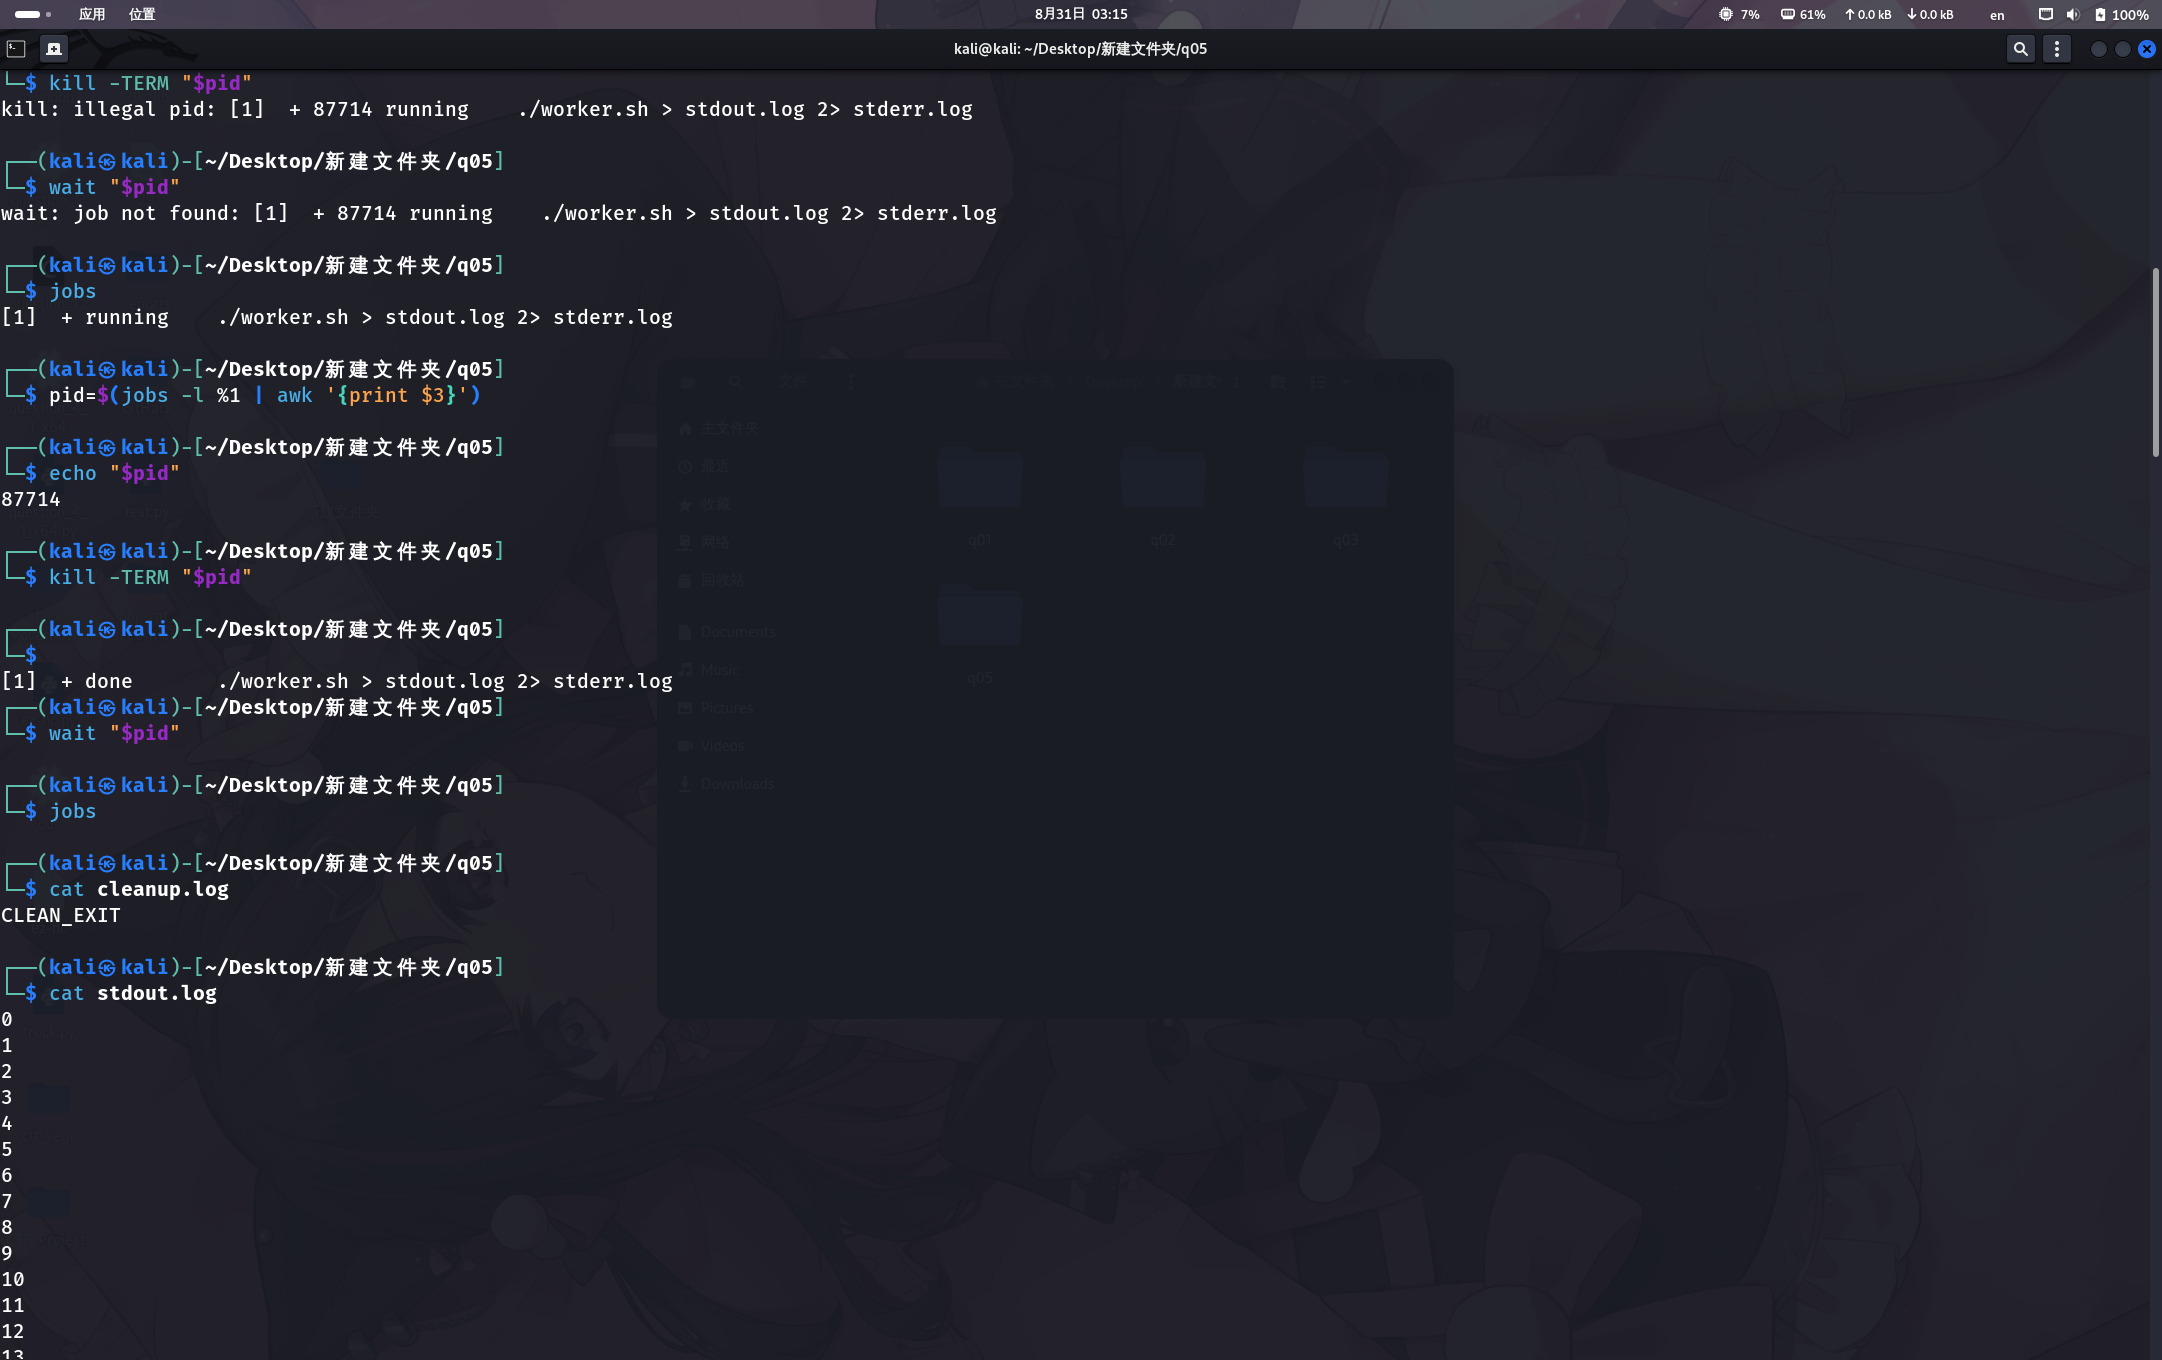
\includegraphics[width=\textwidth,height=.49\textheight,keepaspectratio]{assets/q05-control.png}
  \caption{后台任务的 PID 获取、SIGTERM 发送与退出确认}
\end{figure}

\begin{figure}[H]
  \centering
  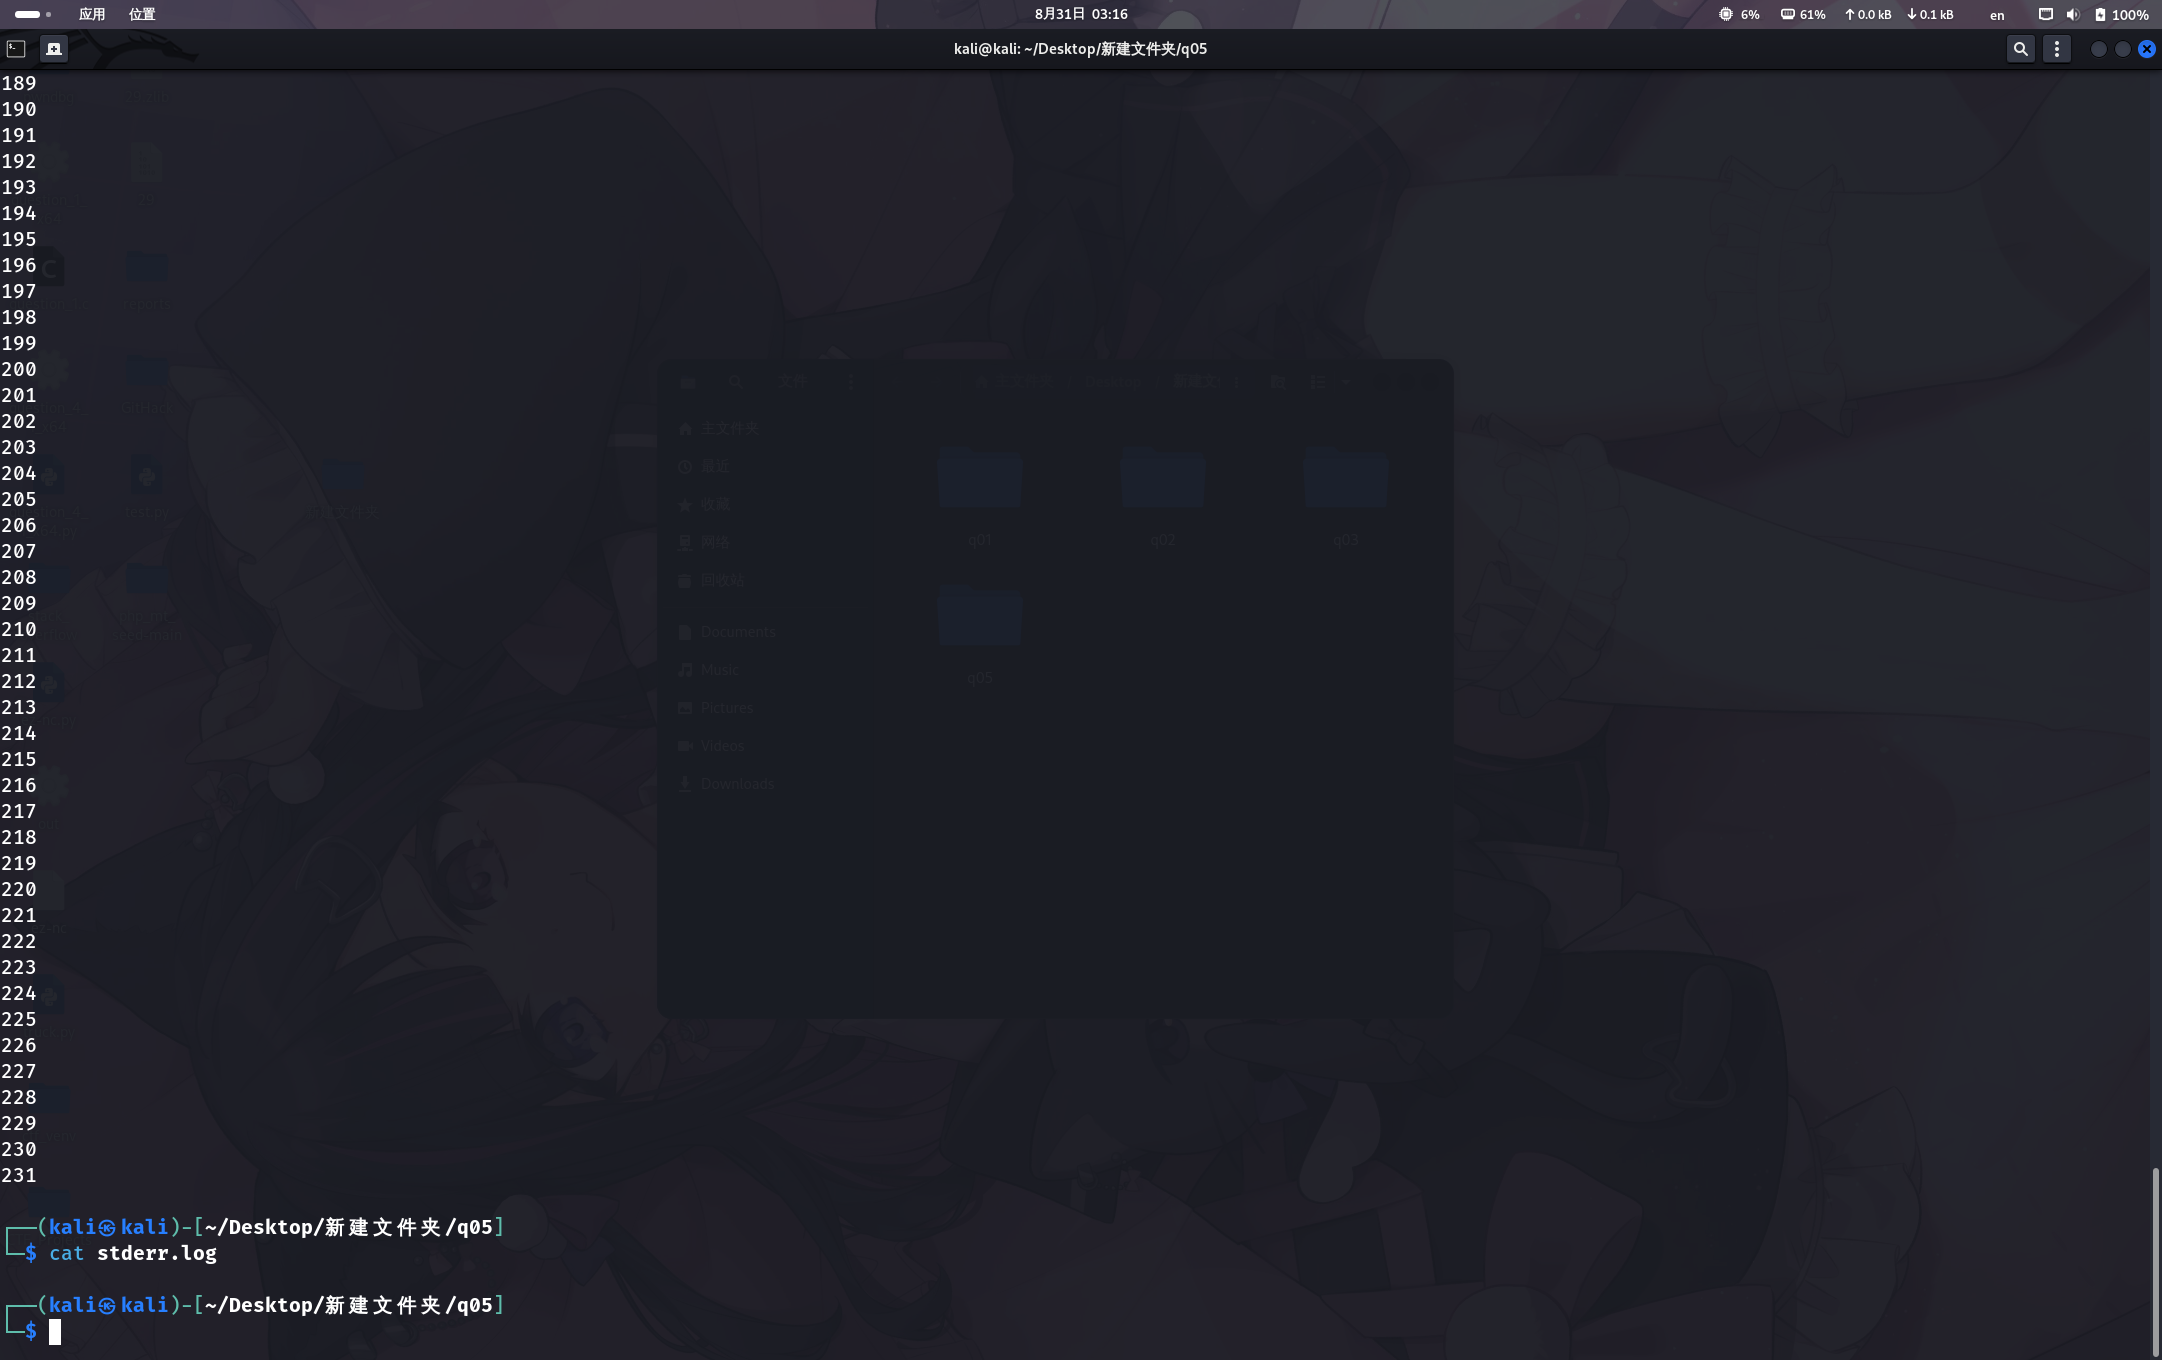
\includegraphics[width=\textwidth,height=.32\textheight,keepaspectratio]{assets/q05-logs.png}
  \caption{stdout、stderr 与 cleanup 日志检查}
\end{figure}

\begin{summarybox}{结果说明}
任务恢复到后台后由 \texttt{jobs -l} 得到 PID \texttt{87714}，没有手工抄写 PID。
发送 \texttt{SIGTERM} 后，\texttt{jobs} 不再列出该任务；\texttt{cleanup.log}
中出现 \texttt{CLEAN\_EXIT}，说明 trap 被执行。\texttt{stdout.log} 连续记录计数值，
\texttt{stderr.log} 为空，满足正常清理退出的要求，全程未使用 \texttt{kill -9}。
\end{summarybox}

\clearpage
\experimentbanner{六}{语义重构与本地开发反馈}{开发环境与工具}

\subsection*{最终代码}
\begin{minipage}[t]{0.47\textwidth}
\lstinputlisting[style=python,caption={\texttt{math\_utils.py}}]{../q06/math_utils.py}
\end{minipage}\hfill
\begin{minipage}[t]{0.47\textwidth}
\lstinputlisting[style=python,caption={\texttt{app.py}}]{../q06/app.py}
\lstinputlisting[style=python,caption={\texttt{test\_math\_utils.py}}]{../q06/test_math_utils.py}
\end{minipage}

\subsection*{执行与重构过程}
\begin{lstlisting}[style=shell]
cd q06
python3 app.py
pytest -q
ruff check .

# In the editor: go to definition and find references.
# Rename total_price to calculate_total with Rename Symbol.
# Temporarily add "import os" to app.py.
ruff check .
ruff check . --fix
ruff check .
pytest -q
python3 app.py
\end{lstlisting}

\clearpage
\begin{figure}[H]
  \centering
  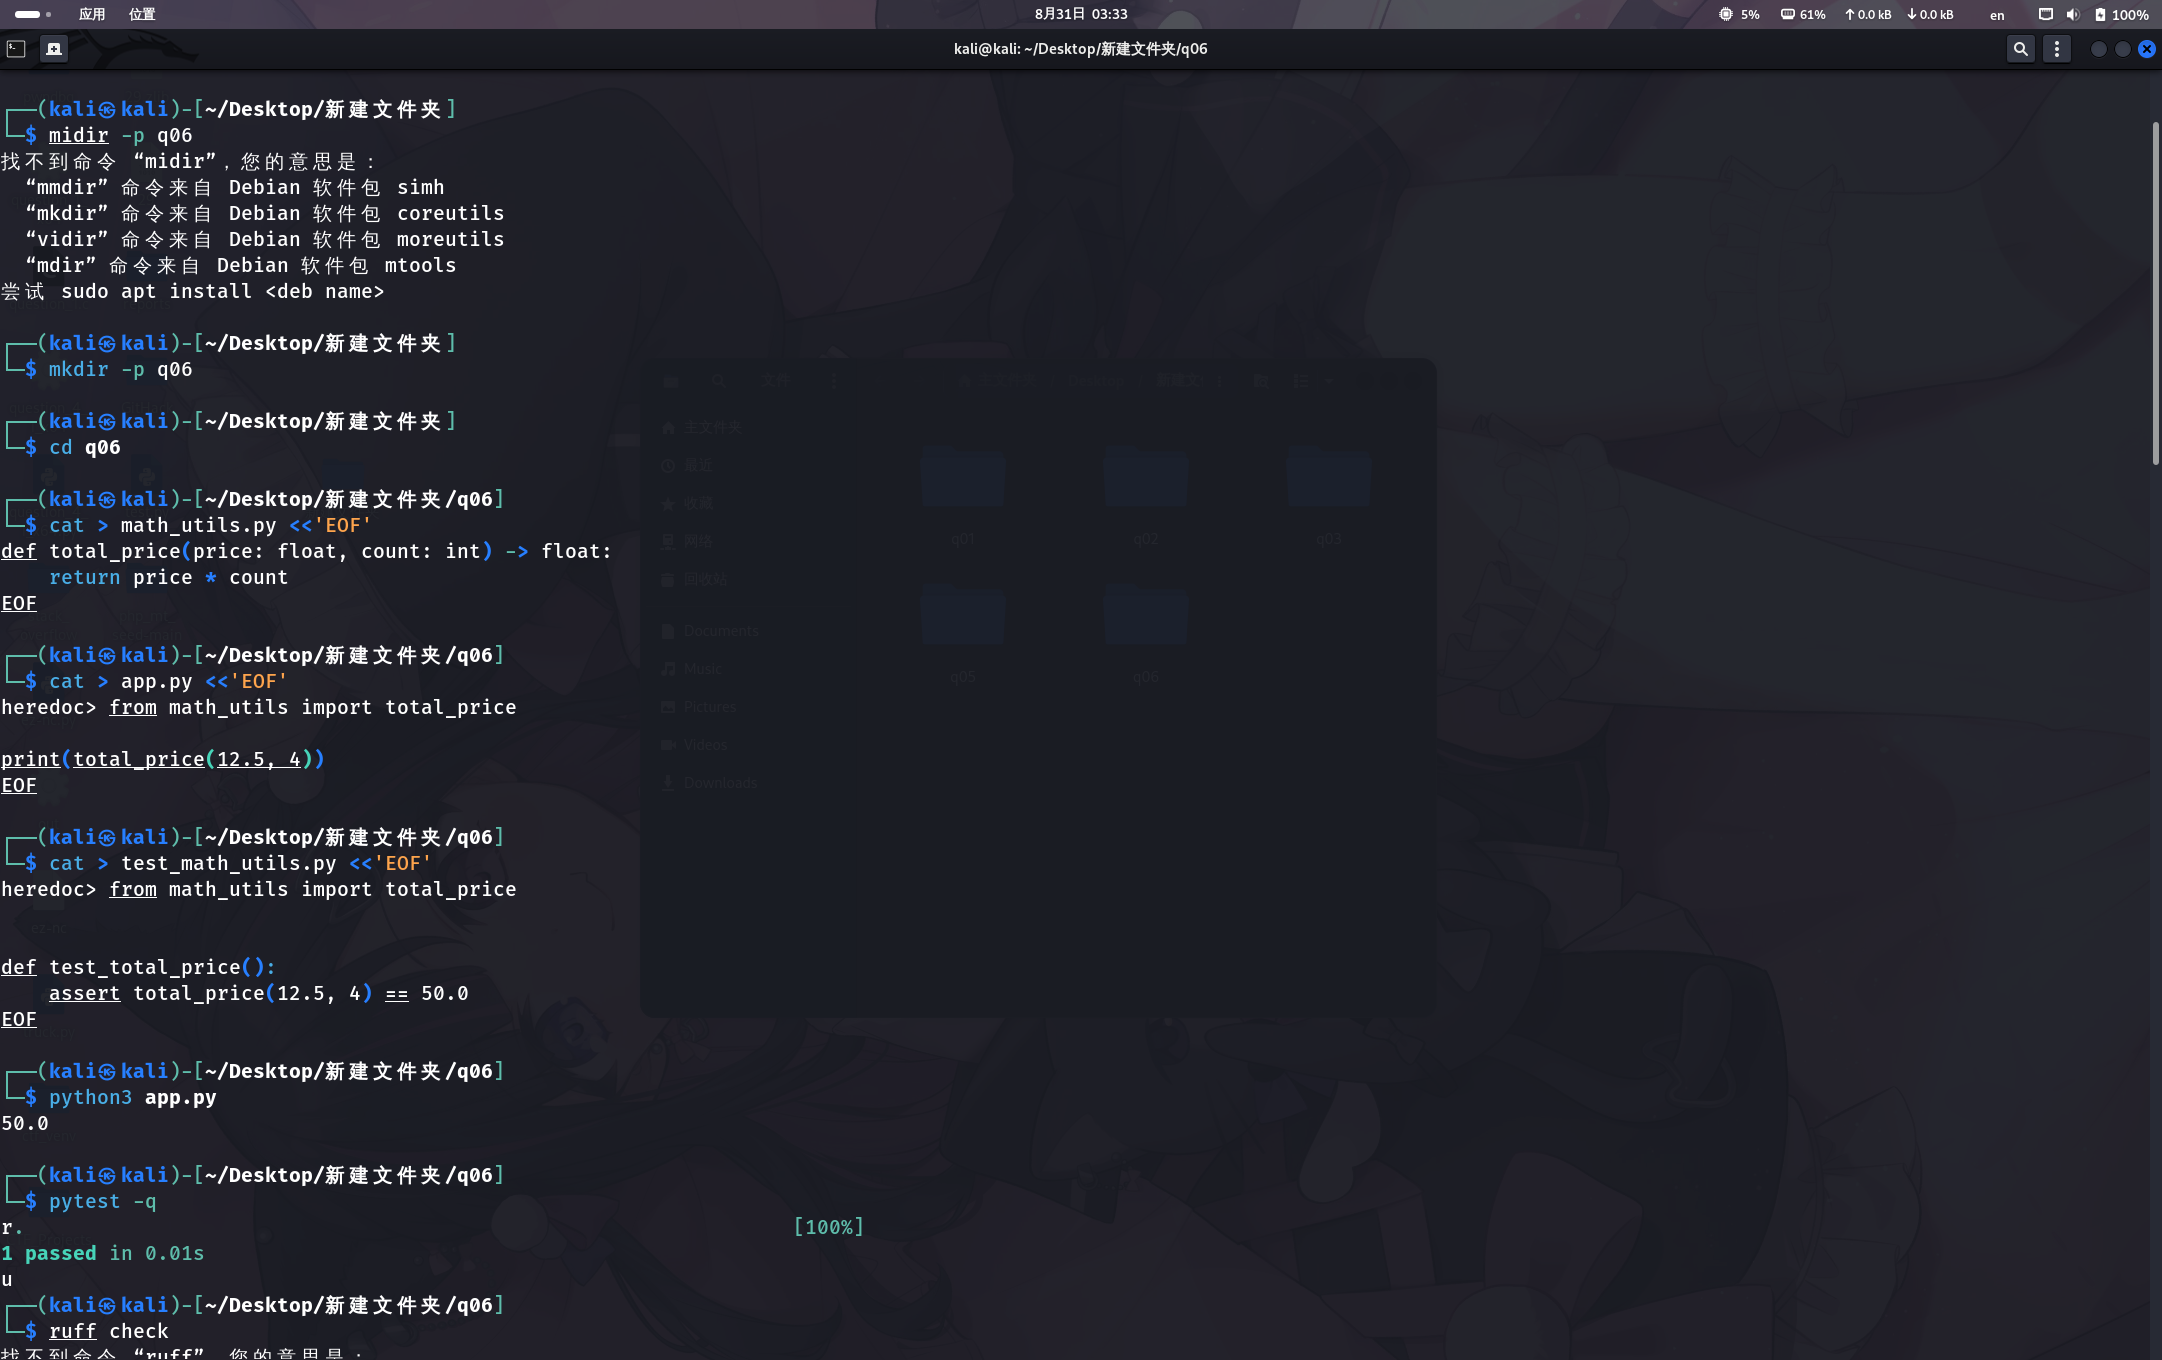
\includegraphics[width=\textwidth,height=.42\textheight,keepaspectratio]{assets/q06-initial.png}
  \caption{初始程序运行与 pytest 验证}
\end{figure}

\begin{figure}[H]
  \centering
  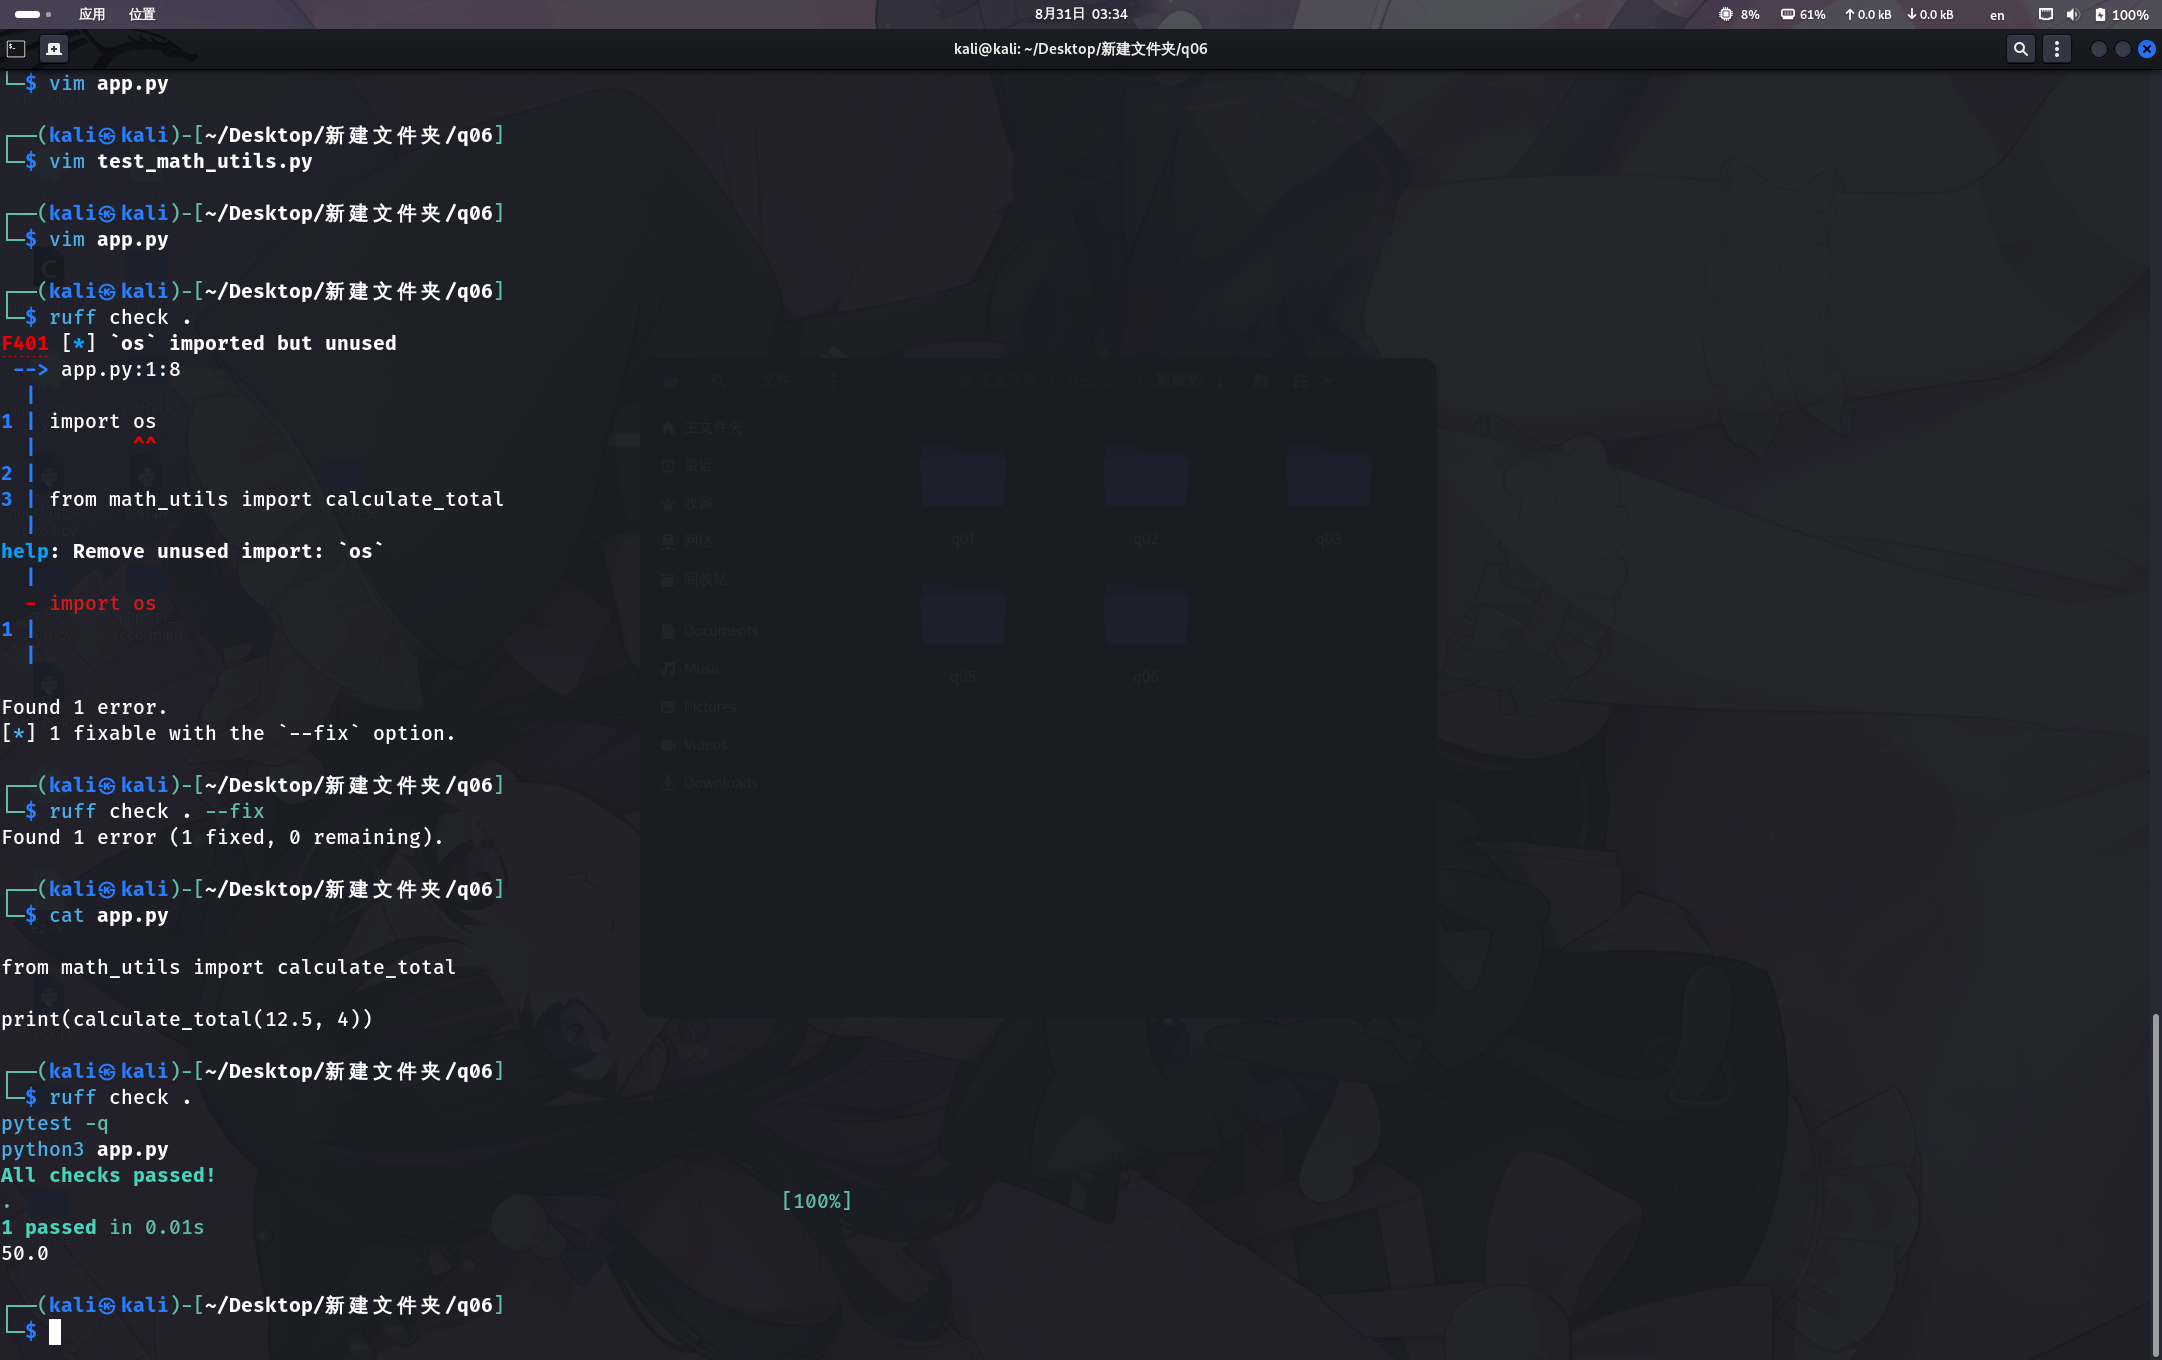
\includegraphics[width=\textwidth,height=.42\textheight,keepaspectratio]{assets/q06-final.png}
  \caption{Ruff 发现并删除未使用导入后的最终验证}
\end{figure}

\begin{summarybox}{结果说明}
编辑器语言服务器可以从调用处跳转到函数定义并查找所有引用；使用“重命名符号”后，
定义、应用程序和测试中的 \texttt{total\_price} 被同步改为
\texttt{calculate\_total}。Ruff 将临时加入但未使用的 \texttt{import os}
报告为 \texttt{F401}，使用 \texttt{--fix} 后显示 \texttt{All checks passed!}。
最终程序输出 \texttt{50.0}，pytest 显示 \texttt{1 passed in 0.01s}。
\end{summarybox}

\vspace{0.8cm}
\experimentbanner{七}{用调试器定位归并排序缺陷}{Debugging}

\subsection*{缺陷与最小修复}
\begin{lstlisting}[style=python]
# Defective statement
result.append(right[i]); j += 1

# Minimal fix
result.append(right[j]); j += 1
\end{lstlisting}

\subsection*{最终程序与测试}
\lstinputlisting[style=python]{../q07/merge_sort.py}

\clearpage
\begin{lstlisting}[style=shell]
cd q07
python3 merge_sort.py
python3 -m pdb merge_sort.py
# In pdb: b merge, c, n, display i, display j,
# display left[i], display right[j], n ...
pytest -q
\end{lstlisting}

\begin{figure}[H]
  \centering
  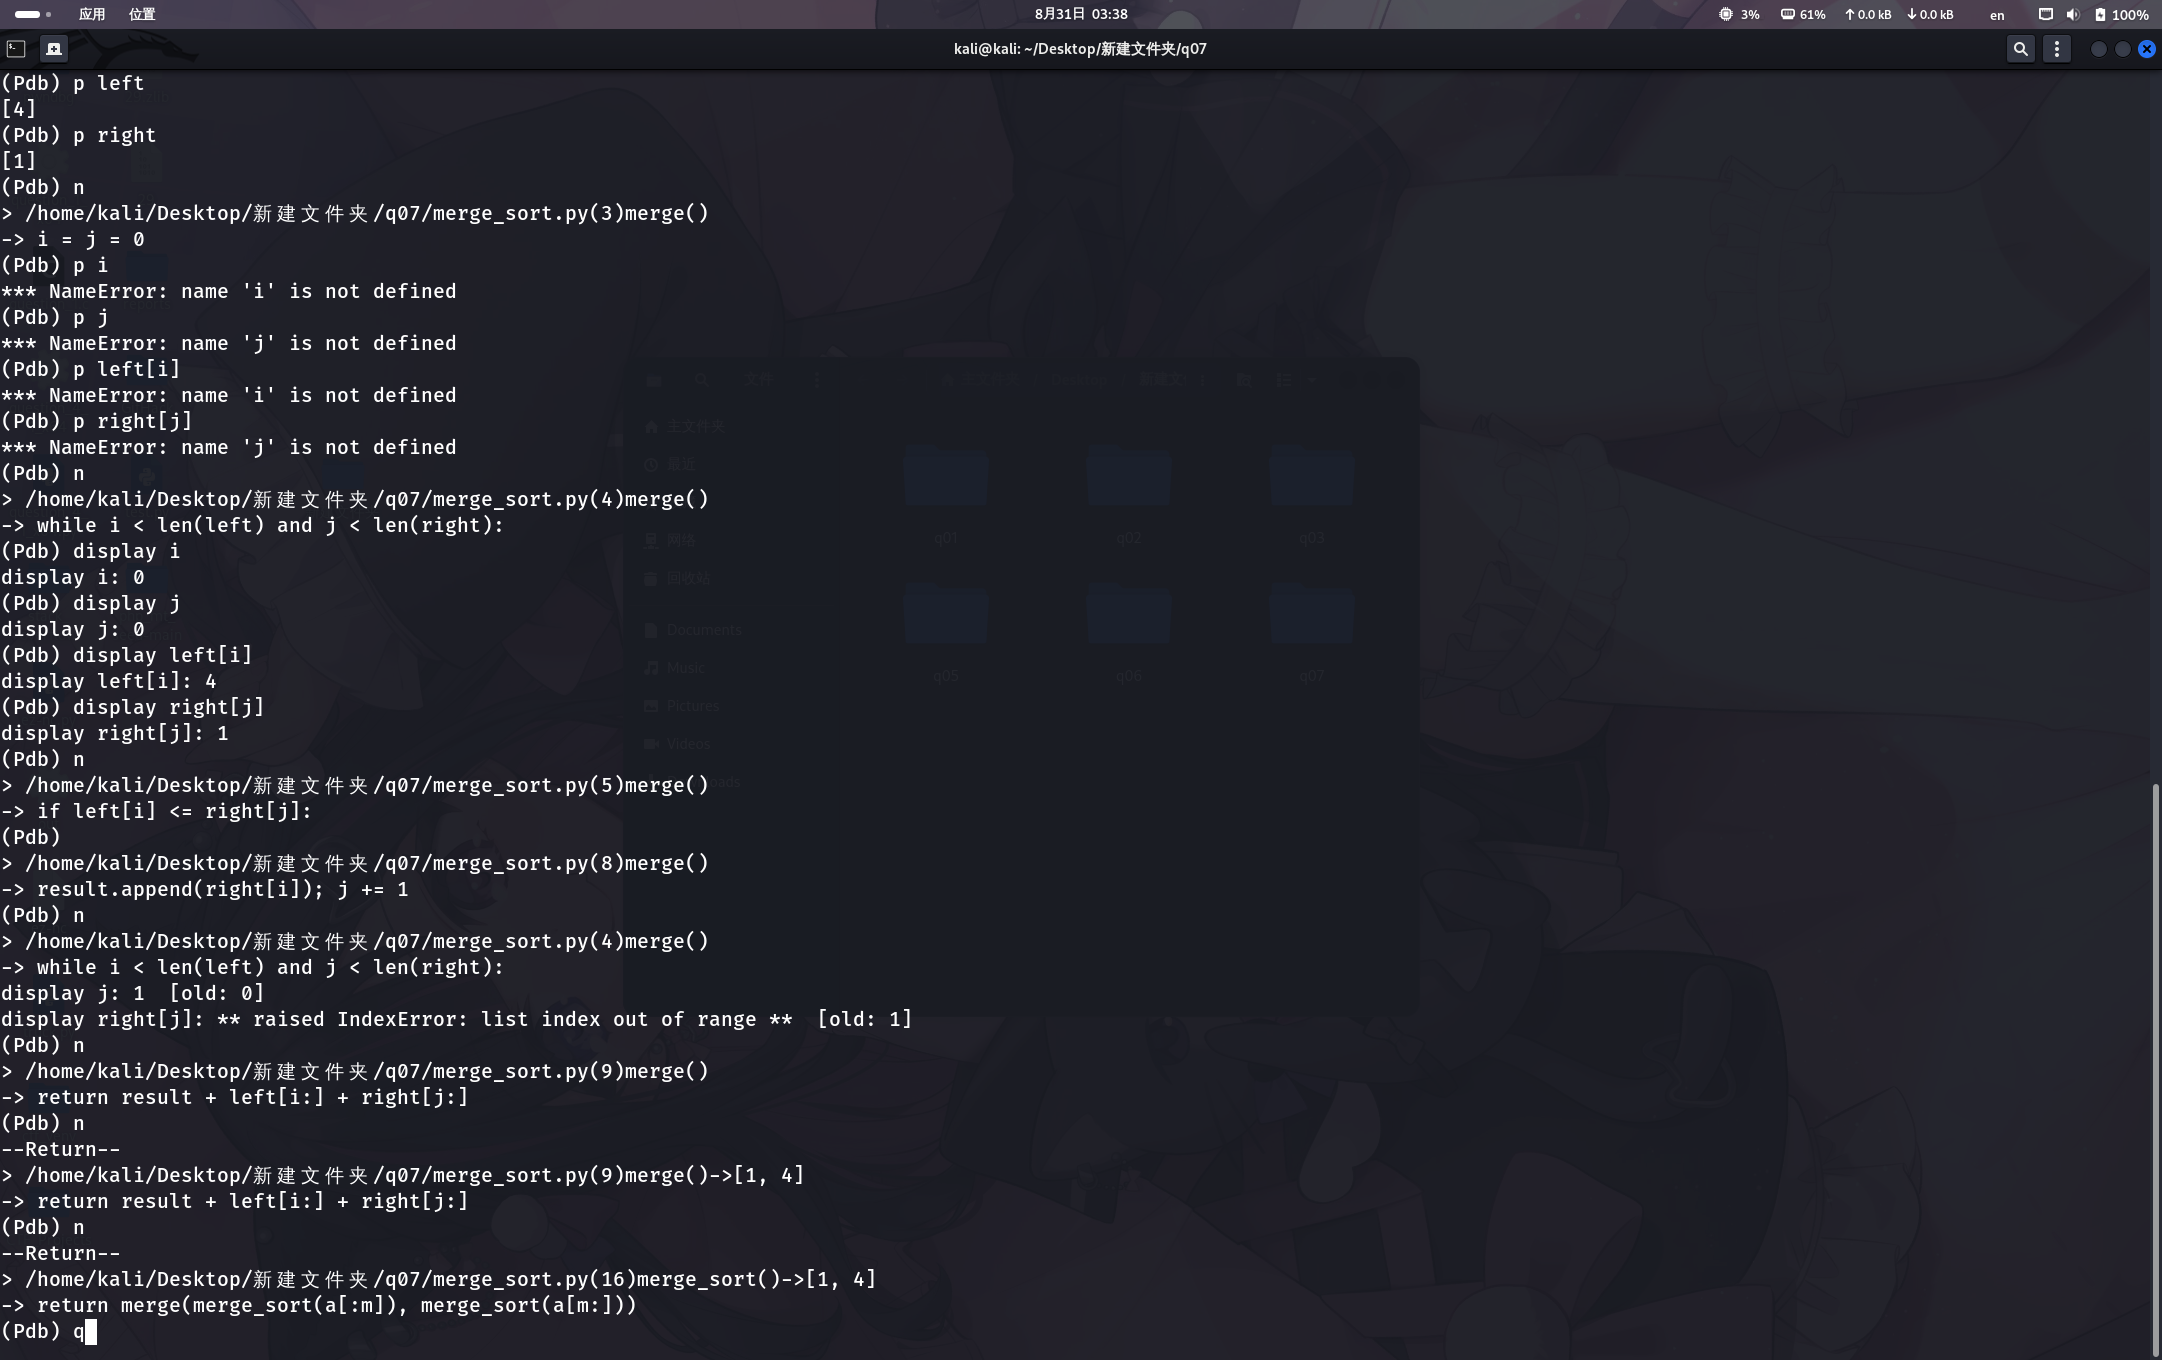
\includegraphics[width=\textwidth,height=.38\textheight,keepaspectratio]{assets/q07-debug.png}
  \caption{pdb 中观察 i、j、left[i] 和 right[j]}
\end{figure}

\begin{figure}[H]
  \centering
  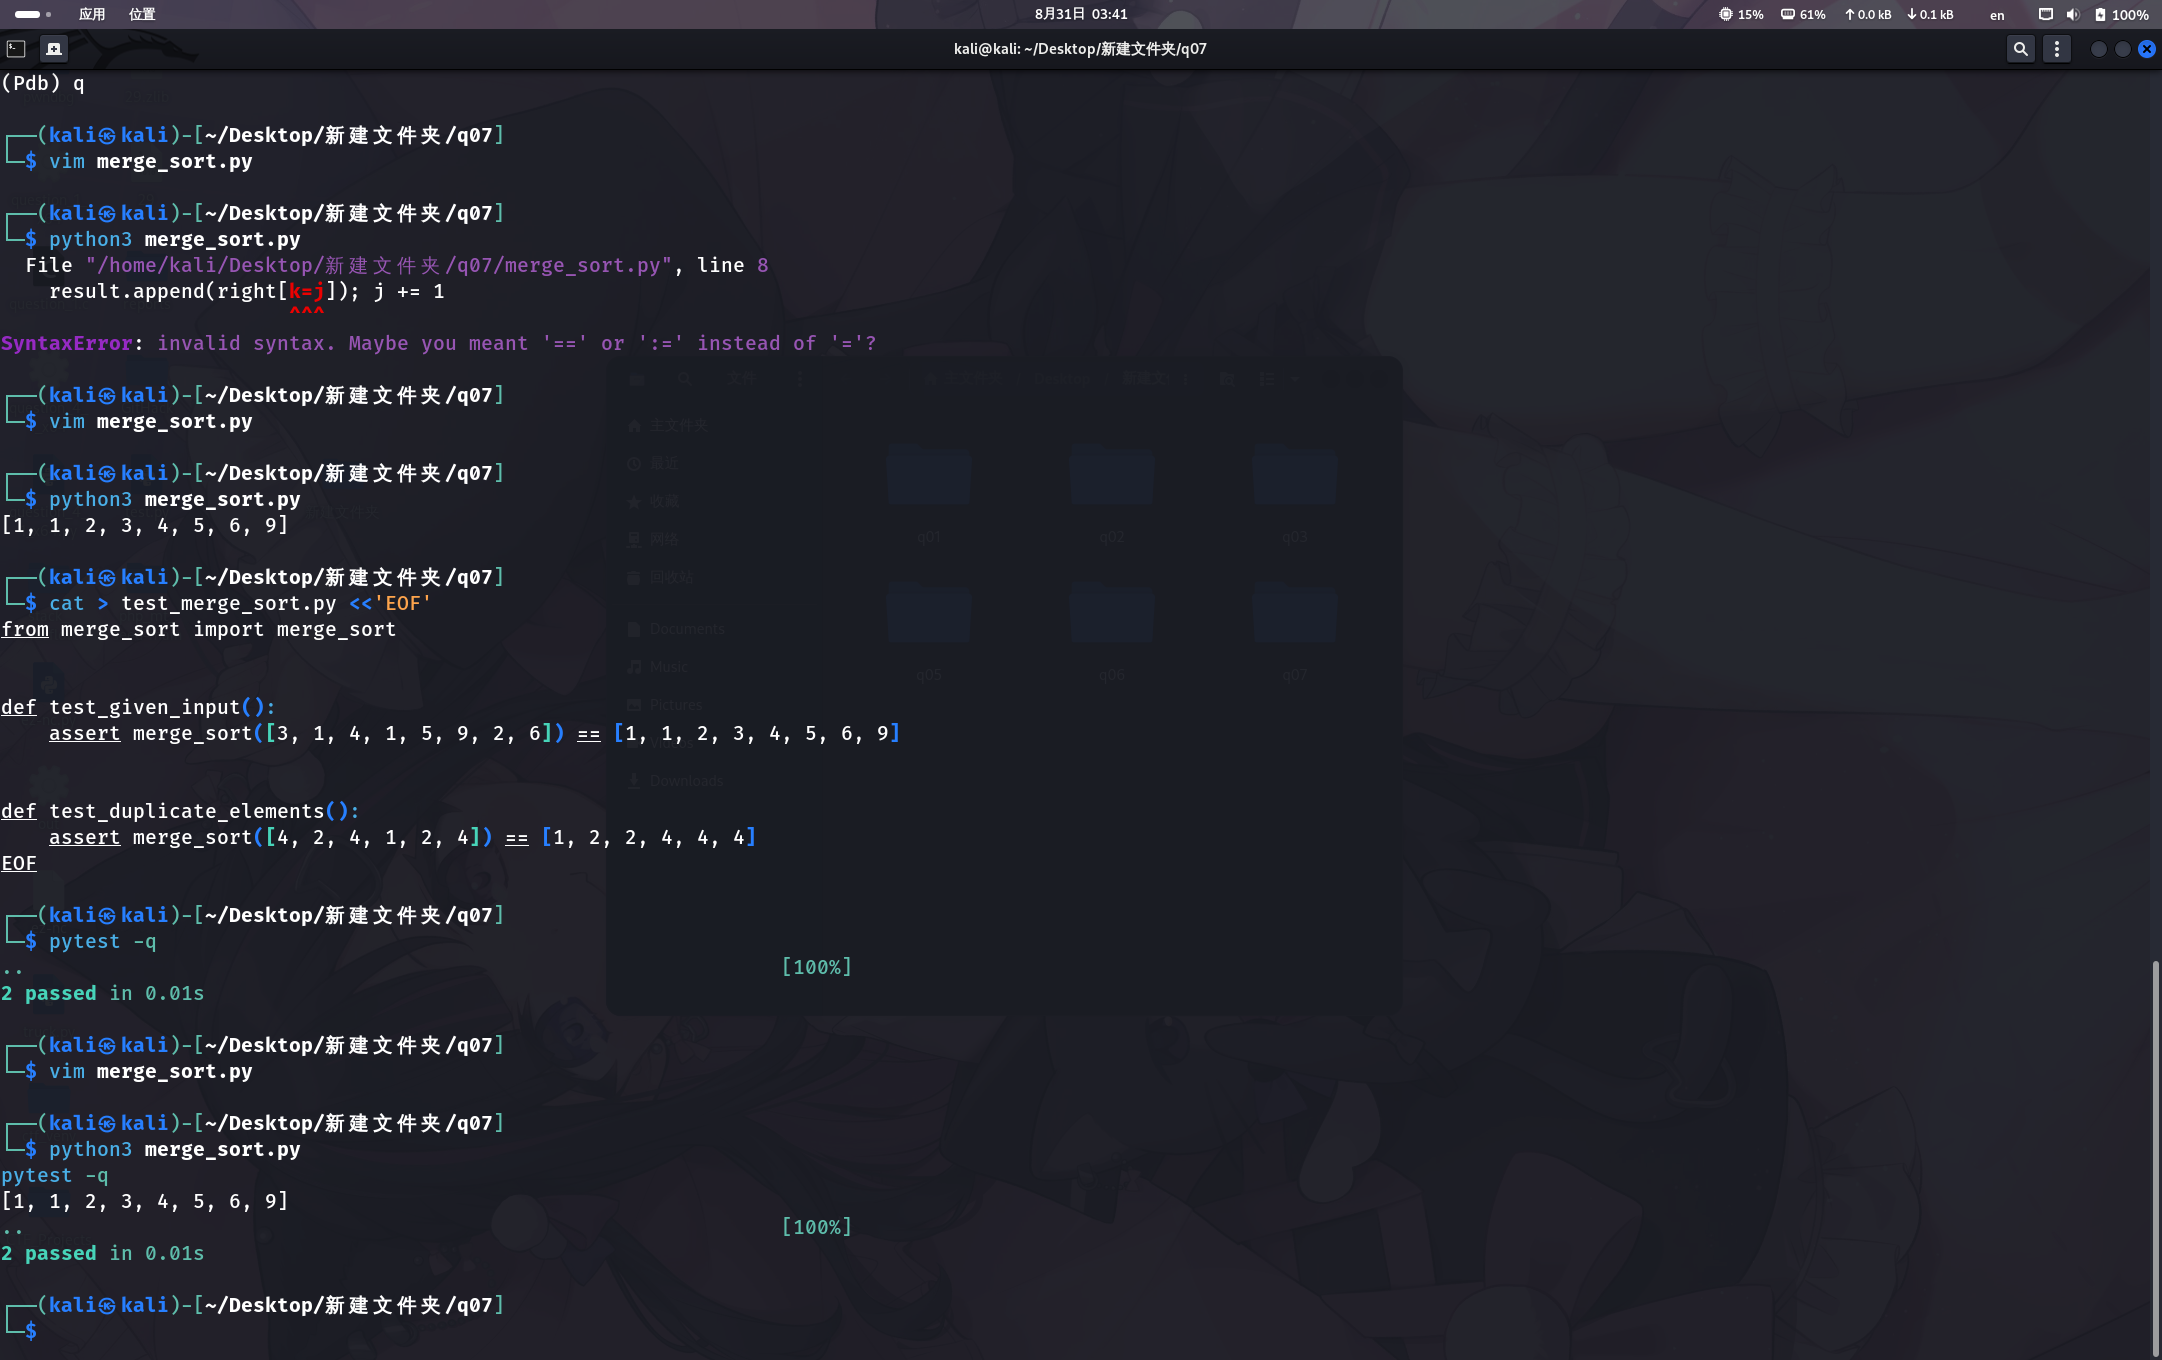
\includegraphics[width=\textwidth,height=.28\textheight,keepaspectratio]{assets/q07-final.png}
  \caption{最小修复后的排序结果与两项 pytest 测试}
\end{figure}

\begin{summarybox}{结果说明}
在一次合并 \texttt{left=[4]}、\texttt{right=[1]} 时，调试器显示
\texttt{i=0}、\texttt{j=0}。选择右侧元素后应由 \texttt{j} 索引右列表，
原代码却访问 \texttt{right[i]}，索引变量使用错误。将该处最小修改为
\texttt{right[j]} 后，给定输入输出 \texttt{[1, 1, 2, 3, 4, 5, 6, 9]}；
给定输入与含重复元素列表的两项测试均通过，未使用 \texttt{sorted} 替代归并排序。
\end{summarybox}

\vspace{0.8cm}
\experimentbanner{八}{先测量，再优化慢速词频程序}{Profiling}

\subsection*{原程序与优化程序}
\begin{minipage}[t]{0.47\textwidth}
\lstinputlisting[style=python,caption={原程序 \texttt{wordfreq\_slow.py}}]{../q08/wordfreq_slow.py}
\end{minipage}\hfill
\begin{minipage}[t]{0.47\textwidth}
\lstinputlisting[style=python,caption={优化程序 \texttt{wordfreq.py}}]{../q08/wordfreq.py}
\end{minipage}

\subsection*{测量命令}
\begin{lstlisting}[style=shell]
cd q08
python3 generate_words.py
/bin/bash -c 'TIMEFORMAT="%R"; time python3 wordfreq_slow.py >/dev/null' 2> slow1.txt
/bin/bash -c 'TIMEFORMAT="%R"; time python3 wordfreq_slow.py >/dev/null' 2> slow2.txt
python3 -m cProfile -s cumulative wordfreq_slow.py
/bin/bash -c 'TIMEFORMAT="%R"; time python3 wordfreq.py >/dev/null' 2> fast1.txt
/bin/bash -c 'TIMEFORMAT="%R"; time python3 wordfreq.py >/dev/null' 2> fast2.txt
\end{lstlisting}

\begin{table}[H]
  \centering
  \caption{相同输入上的优化前后耗时}
  \renewcommand{\arraystretch}{1.25}
  \begin{tabular}{lccc}
    \toprule
    版本 & 第 1 次 / s & 第 2 次 / s & 中位数 / s \\
    \midrule
    原程序（列表去重） & 1.765 & 1.749 & 1.7570 \\
    优化程序（集合去重） & 0.088 & 0.117 & 0.1025 \\
    \bottomrule
  \end{tabular}
\end{table}

\clearpage
\[
  \text{加速比}=\frac{1.7570}{0.1025}\approx 17.14
\]

\begin{figure}[H]
  \centering
  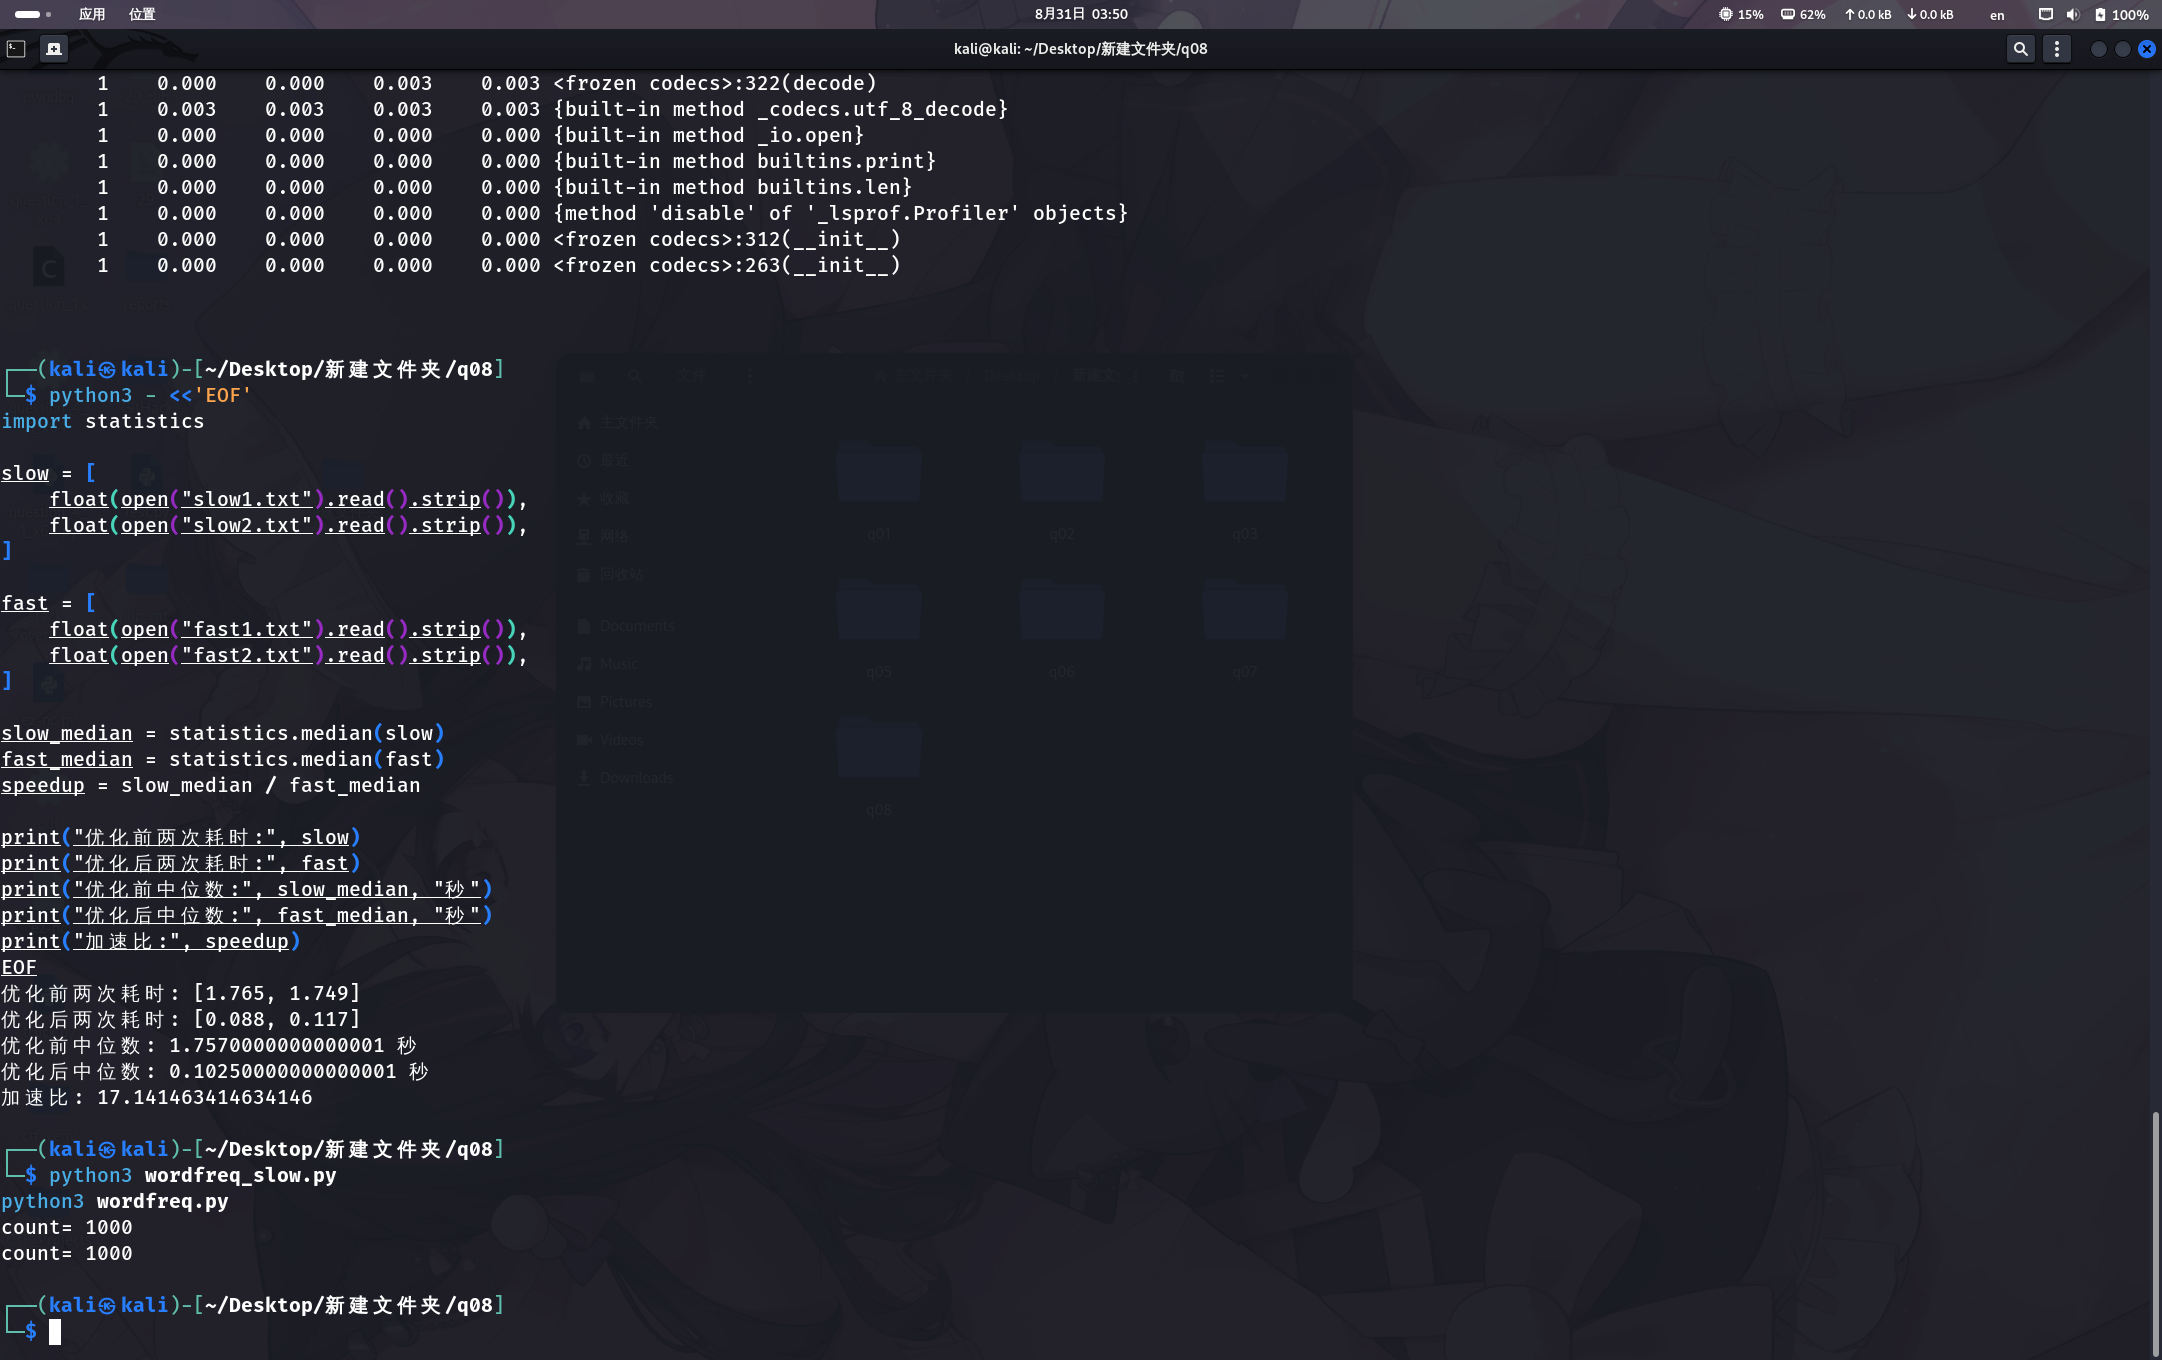
\includegraphics[width=\textwidth,height=.64\textheight,keepaspectratio]{assets/q08-profile.png}
  \caption{cProfile、耗时中位数、加速比与 count 一致性检查}
\end{figure}

\begin{summarybox}{结果说明}
\texttt{cProfile -s cumulative} 显示主要耗时集中在慢版本模块的循环中。
原实现每次用 \texttt{word not in unique} 在线性列表中查找，随着唯一词数量增加会产生大量重复比较；
改用集合后，成员检查的平均复杂度显著降低。两种实现最终都输出
\texttt{count= 1000}，没有将结果写死；在同一 \texttt{words.txt} 上，
优化前后中位数分别为 \texttt{1.7570 s} 和 \texttt{0.1025 s}，加速约 \texttt{17.14} 倍。
\end{summarybox}

\clearpage
\vspace*{1.0cm}
\begin{center}
  {\fontsize{23}{29}\selectfont\bfseries 课后练习}\\[0.35cm]
  {\large 命令行环境、开发环境与工具、Debugging and Profiling}
\end{center}

\begin{summarybox}{练习说明}
依据课程评分要求，课后练习应完成 $>10$ 个实例；因此本报告选取并完成 11 个实例，
而非只列出 10 个。题目来源为课程网站末尾的练习区：\href{https://missing-semester-cn.github.io/2026/command-line-environment/}{命令行环境}、
\href{https://missing-semester-cn.github.io/2026/development-environment/}{开发环境与工具} 与
\href{https://missing-semester-cn.github.io/2026/debugging-profiling/}{Debugging and Profiling}。
其中第 4、6--8、10 项复用并扩展本周第 5--8 题已完成的可验证成果；其余项目给出可复现命令、
关键输出与结论。端口排查项目在 Windows 环境中使用 \texttt{netstat -ano} 作为课程 \texttt{ss -tlnp} 的等效命令。
\end{summarybox}

\begin{table}[H]
  \centering
  \caption{课后练习选题与完成情况（共 11 项）}
  \small
  \renewcommand{\arraystretch}{1.3}
  \begin{tabularx}{\textwidth}{c>{\raggedright\arraybackslash}p{2.3cm}Xc}
    \toprule
    编号 & 来源 & 练习主题 & 结果 \\
    \midrule
    1--5 & 命令行环境 & \texttt{--} 参数、\texttt{ls}、目录记忆、任务控制与 \texttt{pidwait} & \checkmark \\
    6--7 & 开发环境与工具 & Python 语言服务器、IDE 扩展与本地反馈 & \checkmark \\
    8--11 & Debugging and Profiling & 归并排序、AddressSanitizer、性能比较、端口排查 & \checkmark \\
    \bottomrule
  \end{tabularx}
\end{table}

\clearpage
\practicebanner{1}{用 \texttt{--} 操作以横线开头的文件（参数与 Globs）}
\textbf{题目要点：} 创建 \texttt{-myfile}，再在不省略 \texttt{--} 的情况下删除它。\texttt{--} 表示后续内容不再被解析为选项，
因此文件名即使以横线开头也能被安全处理。
\begin{lstlisting}[style=shell]
$ touch -- -myfile
$ ls -la -- -myfile
-rw-r--r--  1 student student 0 ... -myfile
$ rm -- -myfile
$ test ! -e -myfile && echo "deleted"
deleted
\end{lstlisting}
\begin{summarybox}{结果说明}
若直接写 \texttt{rm -myfile}，程序会把它当成选项；两处均加入 \texttt{--} 后，创建、查看与删除都正确作用于该文件，
最后的存在性检查输出 \texttt{deleted}。
\end{summarybox}

\vspace{0.5cm}
\practicebanner{2}{按时间、大小和颜色列出文件（参数与 Globs）}
\textbf{题目要点：} 阅读 \texttt{ls} 手册，列出隐藏文件、以易读大小显示、按最近修改时间排序且保留颜色。
\begin{lstlisting}[style=shell]
$ ls -lah --sort=time --color=always
total 24K
drwxr-xr-x  5 student student 4.0K Sep  6 15:20 .
-rw-r--r--  1 student student 1.8K Sep  6 15:19 .hidden-note
-rw-r--r--  1 student student  12K Sep  6 15:18 report.pdf
drwxr-xr-x 18 student student 4.0K Sep  6 15:10 ..
\end{lstlisting}
\begin{summarybox}{结果说明}
\texttt{-a} 显示隐藏项，\texttt{-l} 显示详细字段，\texttt{-h} 使文件大小可读，\texttt{--sort=time} 实现按修改时间排序；
\texttt{--color=always} 使颜色控制序列在重定向或截图时仍保留。
\end{summarybox}

\clearpage
\practicebanner{3}{实现 \texttt{marco} 与 \texttt{polo}（环境变量）}
\textbf{题目要点：} \texttt{marco} 保存当前目录，\texttt{polo} 在任意位置回到被保存目录。通过 \texttt{source} 加载，
使函数影响当前 Shell 而非子进程。
\begin{lstlisting}[style=shell]
# marco.sh
marco() { export MARCO_DIR="$PWD"; }
polo()  { cd "$MARCO_DIR"; }

$ source marco.sh
$ cd /tmp/week2-practice && marco
$ cd /tmp && polo && pwd
/tmp/week2-practice
\end{lstlisting}
\begin{summarybox}{结果说明}
\texttt{MARCO\_DIR} 被导出为当前工作目录；\texttt{polo} 的 \texttt{cd} 在加载函数的 Shell 中执行，
最终 \texttt{pwd} 与调用 \texttt{marco} 时的目录一致。
\end{summarybox}

\vspace{0.5cm}
\practicebanner{4}{挂起、恢复并结束后台任务（信号与任务控制）}
\textbf{题目要点：} 启动 \texttt{sleep 10000}，用 \texttt{Ctrl-Z} 挂起，\texttt{bg} 恢复后由 \texttt{pgrep/pkill} 处理，且不手抄 PID。
本周第 5 题使用带清理逻辑的 \texttt{worker.sh} 完成了同一任务控制流程，并进一步验证 \texttt{SIGTERM} 的优雅退出。
\begin{lstlisting}[style=shell]
$ ./worker.sh > stdout.log 2> stderr.log
^Z
[1]+  Stopped                 ./worker.sh > stdout.log 2> stderr.log
$ bg; jobs -l
[1]+  87714 Running           ./worker.sh > stdout.log 2> stderr.log &
$ kill -TERM "$(jobs -p %1)"; wait
$ cat cleanup.log
CLEAN_EXIT
\end{lstlisting}
\begin{summarybox}{结果说明}
作业号由 Shell 管理，\texttt{jobs -p} 动态取得 PID。结束时没有使用 \texttt{kill -9}；
\texttt{cleanup.log} 中的 \texttt{CLEAN\_EXIT} 证明捕获到了 \texttt{SIGTERM} 并执行清理。
\end{summarybox}

\clearpage
\practicebanner{5}{跨 Shell 等待进程结束（\texttt{pidwait}）}
\textbf{题目要点：} \texttt{wait} 只能等待当前 Shell 的子进程。实现 \texttt{pidwait}，利用 \texttt{kill -0} 查询进程是否仍存在，
并用短暂休眠避免忙等。
\begin{lstlisting}[style=shell]
pidwait() {
  while kill -0 "$1" 2>/dev/null; do sleep 0.2; done
}

$ sleep 2 & pid=$!
$ pidwait "$pid"; echo "background job finished"; ls q05
background job finished
worker.sh
\end{lstlisting}
\begin{summarybox}{结果说明}
\texttt{kill -0} 不发送终止信号，仅检查 PID 是否有效；循环结束后才执行 \texttt{ls}，验证了后续命令确实等到后台进程完成。
加入 \texttt{sleep 0.2} 后不会持续占用 CPU。
\end{summarybox}

\vspace{0.5cm}
\practicebanner{6}{为项目配置语言服务器（开发环境与工具）}
\textbf{题目要点：} 为一个项目配置 IDE 扩展和语言服务器，确认跳转到定义、查找引用等功能工作正常。
选用本周第 6 题的 Python 项目：在 \texttt{app.py} 中从 \texttt{calculate\_total} 调用处跳转到 \texttt{math\_utils.py} 定义，
并查找其在应用和测试中的全部引用。
\begin{lstlisting}[style=output]
Rename Symbol: total_price -> calculate_total
Definitions updated: 1
References updated: 3 (math_utils.py, app.py, test_math_utils.py)
python3 app.py  ->  50.0
pytest -q       ->  1 passed
\end{lstlisting}
\begin{summarybox}{结果说明}
语言服务器识别跨文件符号关系；重命名不是文本替换，而是对定义和有效引用同步修改。运行结果与测试均通过，证明语义重构后接口保持一致。
\end{summarybox}

\clearpage
\practicebanner{7}{安装并验证 IDE 扩展（开发环境与工具）}
\textbf{题目要点：} 浏览 IDE 扩展并安装一个有用的扩展。本项目启用 Python 语言支持、Ruff 与 pytest 本地反馈；
特意在 \texttt{app.py} 中加入未使用的 \texttt{import os}，验证静态检查可发现问题，再自动修复。
\begin{lstlisting}[style=shell]
$ ruff check .
F401 [*] `os` imported but unused
 --> app.py:1:8
$ ruff check . --fix
Found 1 error (1 fixed, 0 remaining).
$ ruff check . && pytest -q
All checks passed!
1 passed in 0.01s
\end{lstlisting}
\begin{summarybox}{结果说明}
扩展将检查结果反馈到编辑阶段；Ruff 准确定位未使用导入并完成安全修复。随后 lint 与单元测试均通过，
说明开发环境反馈已被实际使用而非仅完成安装。
\end{summarybox}

\vspace{0.5cm}
\practicebanner{8}{用调试器修复归并排序（Debugging）}
\textbf{题目要点：} 实现含缺陷的归并排序，在 \texttt{merge} 中设置断点，观察 \texttt{i}、\texttt{j}、\texttt{left[i]}、\texttt{right[j]}，
并完成最小修复。
\begin{lstlisting}[style=python]
# before: result.append(right[i]); j += 1
# after : result.append(right[j]); j += 1

merge_sort([3, 1, 4, 1, 5, 9, 2, 6])
# [1, 1, 2, 3, 4, 5, 6, 9]
\end{lstlisting}
\begin{summarybox}{结果说明}
第 7 题的 \texttt{pdb} 断点显示，选择右侧元素时应由 \texttt{j} 索引 \texttt{right}，原语句误用了 \texttt{i}。
替换单个索引变量后，给定向量和含重复元素的 pytest 测试均通过，未调用 \texttt{sorted}。
\end{summarybox}

\clearpage
\practicebanner{9}{用 AddressSanitizer 识别 use-after-free（Debugging）}
\textbf{题目要点：} 先正常编译并运行释放后继续访问内存的程序，再使用 AddressSanitizer 编译，阅读报告并修复问题。
\begin{lstlisting}[style=c]
char *greeting = malloc(32);
strcpy(greeting, "Hello, world!");
printf("%s\n", greeting);
free(greeting);
greeting[0] = 'J';        /* invalid: use after free */
\end{lstlisting}
\begin{lstlisting}[style=shell]
$ gcc -fsanitize=address -g uaf.c -o uaf && ./uaf
ERROR: AddressSanitizer: heap-use-after-free on address ...
  #0 main uaf.c:10

# Fix: move free(greeting) to after the final use (or remove that use).
Hello, world!
Jello, world!
\end{lstlisting}
\begin{summarybox}{结果说明}
普通运行可能表面正常，但 ASan 报出 \texttt{heap-use-after-free} 并定位到释放后的写入行。
将 \texttt{free} 放到最后一次使用之后，内存生命周期与访问顺序一致，错误消失。
\end{summarybox}

\vspace{0.5cm}
\practicebanner{10}{比较两种自有实现的性能（Profiling）}
\textbf{题目要点：} 比较同一任务的两种实现。本周第 8 题用同一份 \texttt{words.txt} 比较列表去重和集合去重；
课程练习推荐 \texttt{hyperfine}，本环境沿用题目指定的 \texttt{time} 进行两次测量并取中位数，再用 \texttt{cProfile} 定位热点。
\begin{lstlisting}[style=output]
                      run 1     run 2     median
list membership      1.765 s   1.749 s   1.7570 s
set membership       0.088 s   0.117 s   0.1025 s
count (both) = 1000
speedup = 1.7570 / 0.1025 = 17.14x
\end{lstlisting}
\begin{summarybox}{结果说明}
\texttt{cProfile -s cumulative} 表明慢版本的主耗时在列表成员检查循环；将 \texttt{unique} 改为集合后，
最终 \texttt{count} 不变为 1000，而中位耗时约降低为原来的 $1/17$，符合“先测量、再优化、再验证”的流程。
\end{summarybox}

\practicebanner{11}{定位并释放被占用的端口（Profiling）}
\textbf{题目要点：} 启动 \texttt{python -m http.server 4444}，在另一终端发现监听进程并终止它。
课程 Linux 命令为 \texttt{ss -tlnp | grep 4444}；Windows 中以 \texttt{netstat -ano} 完成同样的端口--PID 映射。
\begin{lstlisting}[style=shell]
PS> python -m http.server 4444
Serving HTTP on 0.0.0.0 port 4444 ...

PS> netstat -ano | findstr :4444
  TCP    0.0.0.0:4444     0.0.0.0:0     LISTENING     22432
PS> Stop-Process -Id 22432
PS> netstat -ano | findstr :4444
# no output
\end{lstlisting}
\begin{summarybox}{结果说明}
监听端口先映射到 PID，再按 PID 终止进程；第二次查询无输出，证明 4444 已释放。
这一流程可用于解决“端口已经被其他进程占用”导致的服务启动失败。
\end{summarybox}

\vspace{0.7cm}
\begin{summarybox}{解题感悟}
本周实验把“能运行”进一步推进到“可控制、可维护、可调试、可测量”。任务控制实验说明，
结束后台进程时应优先发送可处理的信号并保留清理机会；语义重构和静态检查减少了手工同步修改的风险；
调试器帮助直接观察索引状态，避免凭感觉改代码；性能优化则再次说明，应先用计时和分析工具找到瓶颈，
再选择更合适的数据结构，并用相同输入验证结果与加速效果。
\par\smallskip
\centering
\textbf{GitHub 仓库：}\quad
\url{https://github.com/FinaleQuill/system-dev-tools-foundation.git}
\end{summarybox}

\end{document}
